% Thanks to Kevin D. McGrath for the presentation template.
\documentclass[xcolor={dvipsnames,svgnames},hyperref=dvips]{beamer}

% Packages.
\usepackage{graphicx}
\usepackage{amssymb}
\usepackage{amsmath}
\usepackage{amsthm}
\usepackage{url}
\usepackage{pstricks}
\usepackage{pst-node}
\usepackage{listings}

% Code font-size.
\lstset{
	basicstyle=\tiny
}

% Hyperlinks.
\def\name{Wade Cline}
\hypersetup{
  colorlinks = true,
  citecolor = black,
  linkcolor = black,
  urlcolor = black,
  pdfauthor = {\name},
  pdfkeywords = {``computer science'', lug, cryptography, full-disk},
  pdftitle = {Linux Full-Disk Encryption},
  pdfsubject = {Full-Disk Encryption Basics},
  pdfpagemode = UseNone
}

% ???
\usetheme[hideothersubsections]{Hannover}
\usecolortheme{sidebartab}

% Presentation metadata.
\title[Full-Disk Encryption]{}
\author{Wade Cline}
\date{04 March 2014}

\AtBeginSection[]
{
  \begin{frame}<beamer>{Outline}
    \tableofcontents[currentsection]
  \end{frame}
}
\AtBeginSubsection[]
{
  \begin{frame}<beamer>{Outline}
    % \transwipe
    \tableofcontents[currentsection,currentsubsection]
  \end{frame}
}

\begin{document}

% Title.
\begin{frame}
  \titlepage
\end{frame}

% Table of Contents.
\begin{frame}{Outline}
  % \transwipe
  \tableofcontents
  % You might wish to add the option [pausesections]
\end{frame}

\section{Basics}\label{section:basics}
	\subsection{Terminology}
	\begin{frame}
		\frametitle{Plaintext vs. Ciphertext}
		\begin{itemize}
		\item Plaintext: Unencrypted data.
		\item Ciphertext: Encrypted data.
		\end{itemize}
	\end{frame}

	\begin{frame}[fragile]
		\frametitle{Example Plaintext}
		\begin{itemize}
		\item 512-byte block-file of mostly 0's with a quote at the beginning. \\
		\begin{lstlisting}
		0000000   "   I   t       i   s       s   h   o   c   k   i   n   g    
		0000020   t   o       f   i   n   d       h   o   w       m   a   n   y
		0000040       p   e   o   p   l   e       d   o       n   o   t       b
		0000060   e   l   i   e   v   e       t   h   e   y       c   a   n    
		0000100   l   e   a   r   n   ,       a   n   d       h   o   w       m
		0000120   a   n   y       m   o   r   e       b   e   l   i   e   v   e
		0000140       l   e   a   r   n   i   n   g       t   o       b   e    
		0000160   d   i   f   f   i   c   u   l   t   .   "  \n  \0  \0  \0  \0
		0000200  \0  \0  \0  \0  \0  \0  \0  \0  \0  \0  \0  \0  \0  \0  \0  \0
		*
		0001000
		\end{lstlisting}
		\end{itemize}
	\end{frame}

	\begin{frame}[fragile]
		\frametitle{Example Ciphertext}
		\begin{itemize}
		\item Previous 512-byte block-file encrypted\footnote{\texttt{cryptsetup create --cipher aes-xts-essiv:sha256} with password ``password''} \\
		\begin{lstlisting}
		0000000   N   7 207 374 373   z 244 036 246 232 263 214 202   z 307 216
		0000020 201 251 034 271   1 244 261   C 325 377 333 276 223 003 310 367
		0000040   "   D 232 230 314   B 331 254 365 373 340 352 231 255 355 240
		0000060   { 332 006 333 202 317   r  \f   @ 321   > 302   . 177   D   V
		0000100   q   T 016 345 275 032 377 306   '   7 264 207   D 245 370 363
		0000120   )   u   a 025   > 330 266   I 035 247 372 327 262   s   H   >
		0000140 236 241 300 245 366   , 352 347   k 241   V  \n  \a 260   S   f
		0000160 327   f 022   d   R 375 234 306 020   L 270 035 234 237 320 354
		0000200 020 244   a 333 235 216 336  \n 021 352 264   & 234 334   T 220
		0000220   u 363   \ 334 327   7  \a   j 347 332  \b   7   - 247 214 205
		0000240   t 360   C   ( 204 363 031   l 325 313 306   .  \0 354 036    
		0000260 305 250   Q  \f 374   y 253   ` 370 021 020   \   `   V 213   0
		0000300 212 305 237 262   a   !   X 323 317 254   0 345   D   3   > 323
		0000320   *  \0 005 276   # 222 340   #   t 245   u 251 362 304 231   ]
		0000340   $ 253   & 272   c 311   b 031 033   P 352 366   % 365   -   <
		0000360 246 354 245 361 206 364 332 311   _ 006 374 373 377   {   w   :
		0000400   - 262 214   I 303 223   M   J 256 354 341 004 024   U   & 320
		0000420   { 271   y   G   ' 264   =   E  \r   1   I   `   >   y   = 207
		0000440 335 323   )   I   " 274   2 276   O   ] 240   `   Y 237   & 342
		0000460 351   _ 262 201   J 361 310 002 203  \t 362 260 017 344 205   :
		0000500   ` 377 216  \a 223   F 362   ) 233 243 036 376 340   I 202   S
		\end{lstlisting}
		{\tiny \ldots (truncated for brevity)}
		\end{itemize}
	\end{frame}

	\begin{frame}
		\frametitle{Symmetric Cryptography}
		\begin{itemize}
		\item Same key used to encrypt plaintext and to decrypt ciphertext. 
		\item Useful when only one person needs access to information.
		\item Relevant to today's discussion.
		\item Contrasted with Asymetric Cryptography.
		\item Examples: AES, Blowfish, 3DES, Serpent, Twofish.
		\end{itemize}
	\end{frame}

	\begin{frame}
		\frametitle{Asymetric Cryptography}
		\begin{itemize}
		\item AKA Public-Private Key Cryptography.
		\item Different keys used to encrypt plaintext and to decrypt ciphertext.
		\item Useful when communicating securely between two people.
		\item Contrasted with Symmetric Cryptography.
		\item Example: RSA, SSL.
		\end{itemize}
	\end{frame}

	\begin{frame}
		\frametitle{Block vs. Stream Ciphers}
		\begin{itemize}
		\item Block Ciphers operate on larged, fixed-length chunks of bits.
		\item Stream Ciphers encrypt digits one-at-a-time.
		\item Similar to Block vs. Character Devices.
		\item Block Ciphers relevant to today's discussion.
		\end{itemize}
	\end{frame}

	\subsection{Physical Media}
	\begin{frame}
		\frametitle{Disk Layout}
		\begin{itemize}
		\item Linux divides disks into 512-byte sections known as \textit{sectors}.
		\item Filesystem divides read/writes into \textit{blocksize} units (multiple of sector size).
		\item Encrypted on sector-level, though filesystem may do block-level writes.
		\item Block Cipher size $\leq$ Sector size $\leq$ Block size
			\begin{itemize}
			\item Common values: 128 \textit{bits} - 512 \textit{bytes} - 4096 bytes, respectively.
			\end{itemize}
		\end{itemize}
	\end{frame}

	\begin{frame}
		\frametitle{Example of cipher-size, sector-size, and block-size}
		\begin{itemize}
		\item Red blocks show a 128-bit cipher.
		\item Green blocks show a 512-byte sector.
		\item The blue outline shows a 4096-byte block.
		\end{itemize}
		\centering
		\includegraphics[scale=0.065]{images/sizes.ps}
	\end{frame}

	\begin{frame}
		\frametitle{Wear-leveling}
		\begin{itemize}
		\item Attempts to distribute writes evenly across the device.
		\item Helps with device longevity.
		\item Used mostly in USB and SSD devices.
		\item Makes overwriting files difficult.
		\item Emphasizes proactive encryption.
		\end{itemize}
	\end{frame}

\section{Wiping}\label{wiping}
	\begin{frame}
		\frametitle{Naive Wiping}
		\begin{itemize}
		\item Nuke disk \textit{once} with a series of '0's (\texttt{/dev/zero}).
		\item Fast, simple, but leaks data.
		\item Each filesystem has a metaphorical ``fingerprint''.
		\item Labratory forensic analysis may reveal old data (discussed later).
		\end{itemize}
	\end{frame}

	\begin{frame}
		\frametitle{Example Fingerprints}
		\centering
		\begin{itemize}
		\item 1 GB freshly-created filesystems.
		\end{itemize}
		\begin{tabular}{c c c}
		\texttt{ext4} & \texttt{xfs} & \texttt{btrfs} \\
		\protect \includegraphics[scale=0.30]{images/fingerprint_ext4.ps} &
		\protect \includegraphics[scale=0.30]{images/fingerprint_xfs.ps} &
		\protect \includegraphics[scale=0.30]{images/fingerprint_btrfs.ps} \\
		\end{tabular}
	\end{frame}

	\begin{frame}
		\frametitle{Secure Wiping}
		\begin{itemize}
		\item Use cryptographic-grade pseudo-random numbers.
			\begin{itemize}
			\item \texttt{/dev/urandom} should provide a decent stream.
			\item \texttt{/dev/random} in theory better, but in practice you'd be dead before completion.
			\end{itemize}
		\item Wipe multiple times.
			\begin{itemize}
			\item In theory, proper analysis could reveal previous magnetic states.
			\item Government-``recommended'' is 7 times.
			\end{itemize}
		\item Depending on size of drive and computing power this could take days or weeks.
		\end{itemize}
	\end{frame}

\section{Encryption}\label{section:encryption}
	\subsection{Abstraction}
	\begin{frame}
		\frametitle{Ciphers}
		\begin{itemize}
		\item Transforms a chunk of plaintext into ciphertext.
		\item Support must be enabled in the kernel.
		\item Examples: AES, Serpent, Twofish.
		\end{itemize}
	\end{frame}

	\begin{frame}
		\frametitle{Mode of Operation}
		\begin{itemize}
		\item Recall block ciphers work on fixed-length set of bits.
		\item Recall Linux sector size is 512 \textit{bytes}.
		\item Many of today's block ciphers are 128 \textit{bits}.
		\item A \textit{mode of operation} describes how to repeatedly use a block cipher to encrypt a larger area, such as a sector.
		\item Simply breaking apart reveals patterns in data.
		\item Support must be enabled in the kernel.
		\item Examples: CBC, XTS.
		% TODO: Visualization.
		\end{itemize}
	\end{frame}

	\begin{frame}
		\frametitle{Initialization Vector}
		\begin{itemize}
		\item What is the first block chained with? An \textit{initialization vector}.
		\item Part of the Mode of Operation.
		\item Must appear ``random'' to avoid watermarking.
		\item Example: ESSIV.
		\end{itemize}
	\end{frame}

	\begin{frame}
		\frametitle{Keyfiles}
		\begin{itemize}
		\item Instead of passphrase, use a \textit{keyfile}.
		\item Not limited by human memory, fully-random numbers (\texttt{/dev/random}).
		\item For added protection, encrypt keyfile with passphrase.
			\begin{itemize}
			\item Can also protect against keylogging.
			\end{itemize}
		\end{itemize}
	\end{frame}

	\begin{frame}
		\frametitle{Salts}
		\begin{itemize}
		\item \textit{Additional} input to passphrase during hashing.
		\item Ensure \textit{uniqueness} of result.
		\item Protects against Rainbow Tables.
		\end{itemize}
	\end{frame}

	\begin{frame}
		\frametitle{Key-stretching}
		\begin{itemize}
		\item Passphrases usually \textit{hashed} before input into algorithm.
		\item Increase number of hashing \textit{rounds} before input (0.5 - 2 seconds-worth).
		\item Slows down brute-force \& dictionary attacks dramatically.
		\end{itemize}
	\end{frame}

	\subsection{Implementation}
	\begin{frame}
		\frametitle{\texttt{cryptsetup}}
		\begin{itemize}
		\item \texttt{cryptsetup} front-end to kernel crypto API.
		\item Rather than ``encrypt'' function, create abstraction layer over device.
		\item Entries go under the \texttt{/dev/mapper} directory.
		\item For example, use \texttt{/dev/mapper/root} to access an encrypted \texttt{/dev/sda}.
			\begin{itemize}
			\item \texttt{/dev/sda} appears as garbage (because it's encrypted) to anyone looking at it.
			\item \texttt{/dev/mapper/root} looks like a normal hard drive.
			\end{itemize}
		\item Look under \texttt{ps} for \texttt{kworker}.
		\item Support must be enabled in the kernel (\texttt{CONFIG\_DM\_CRYPT)}.
		% TODO: Visualization.
		\end{itemize}
	\end{frame}

	\begin{frame}
		\frametitle{LUKS and \texttt{dm-crypt}}
		\begin{itemize}
		\item Two main modes: LUKS (Linux Unified Key Setup) and ``plain'' \texttt{dm-crypt},
		\item LUKS is feature-rich, \texttt{dm-crypt} is not.
		\item Simplfied: Beginners use LUKS, advanced users \textit{may} wish to use \texttt{dm-crypt}.
		\end{itemize}
	\end{frame}

	\begin{frame}
		\frametitle{LUKS}
		\begin{itemize}
		\item Creates \textit{LUKS header} metadata on disk.
			\begin{itemize}
			\item One or more key-slots.
			\item Cipher/Mode of Operation.
			\item Encrypted keyfile.
			\item Automatic key-stretching.
			\end{itemize}
		\item Wiping out LUKS header makes disc inaccessible.
		\item Clearly a LUKS-encrypted device.
		\end{itemize}
	\end{frame}

	\begin{frame}
		\frametitle{\texttt{dm-crypt}}
		\begin{itemize}
		\item No metadata on-disk.
		\item No key-stretching.
		\item Just mappings!
		\item Re-specify all parameters precisely or get garbage.
		\item Encrypted device, or wiped device?
		\end{itemize}
	\end{frame}

	\begin{frame}
		\frametitle{Multiple Layers}
		\begin{itemize}
		\item Why rely on one cipher that may get cracked?
		\item Make a mapping over the mapping.
			\begin{itemize}
			\item Example: \texttt{/dev/mapper/root -> /dev/mapper/.extra\_layer -> /dev/sda}
			\end{itemize}
		\item Keep adding layers for more security.
		\end{itemize}
	\end{frame}

\section{Early Userspace}\label{section:hell}
	\begin{frame}
		\frametitle{Basics}
		\begin{itemize}
		\item Root filesystem encrypted, how can Linux mount it?
			\begin{itemize}
			\item Create "early userspace" environment to mount root filesystem.
			\end{itemize}
		\item Part of Linux boot process.
		\item Other uses:
			\begin{itemize}
			\item Load firmware.
			\item Mount root filesystem over NFS.
			\end{itemize}
		\item Documentation:
			\begin{itemize}
			\item \texttt{Documentation/early-userspace/README}
			\item \texttt{Documentation/init.txt}
			\item \texttt{Documentation/initrd.txt}
			\end{itemize}
		\end{itemize}
	\end{frame}

	\begin{frame}
		\frametitle{\texttt{initramfs}}
		\begin{itemize}
		\item \texttt{initramfs} contains Early-userspace environment.
		\item Successor to \texttt{initrd}.
		\item Gzipped CPIO archive.
			\begin{itemize}
			\item Magic command: \texttt{find . | cpio --quiet -H newc -o | gzip -9 -n > ../initramfs}
			\end{itemize}
		\item Contains initial root file system \& \texttt{init} script.
		\item Execute \texttt{init} script, which switches to actual root filesystem; early-userspace environment discarded.
		\item Support must be enable in kernel (\texttt{CONFIG\_BLK\_DEV\_INITRD)}.
		\end{itemize}
	\end{frame}

	\begin{frame}
		\frametitle{Early-userspace Binaries}
		\begin{itemize}
		\item Simply copying binaries unlikely to work (\textit{dynamically-linked}).
			\begin{itemize}
			\item \texttt{ldd} shows dynamic-linking dependencies.
			\end{itemize}
		\item Copy all dependencies or make binaries \textit{statically-linked}.
		\item Statically-compiled binaries are \textit{huge}.
		\end{itemize}
	\end{frame}

	\begin{frame}
		\frametitle{\texttt{busybox}}
		\begin{itemize}
		\item Stripped-down Unix toolkit: \texttt{busybox}.
		\item Often used in embedded Linux systems.
		\item Easier than individually adding binaries such as \texttt{cp}, \texttt{ls}, \texttt{rm}, \&c.
		\item Install built-in binaries: \texttt{busybox --install -s}.
		\item Uses different, basic shells; certain \texttt{bash} features unsupported (ex: arrays).
		\end{itemize}
	\end{frame}

	\begin{frame}
		\frametitle{\texttt{init}}
		\begin{itemize}
		\item Does ``whatever'' needs to be done.
		\item May be a binary or a script.
		\item Will receive same arguments as the kernel.
		\item Easy method: find one on the Internet and study/copy it!
		\item Failure will result in a kernel panic.
		\end{itemize}
	\end{frame}

	\begin{frame}
		\frametitle{Summary}
		\begin{itemize}
		\item Create directory structure for \texttt{initramfs}.
		\item Copy statically-linked binaries, or dynamically-linked binaries with dependenices.
		\item Write \texttt{init} script.
		\item Create a Gzipped CPIO archive:
			\begin{itemize}
			\item \texttt{find . | cpio --quiet -H newc -o | gzip -9 -n > ../initramfs}
			\end{itemize}
		\item Add \texttt{initramfs=</path/to/initramfs>} kernel argument or build it into the kernel.
		\end{itemize}
	\end{frame}

	%TODO: "Fun" visualization.

% References.
\section{References}
\begin{frame}
	\frametitle{References}
	\begin{itemize}
	\item Thorough FAQ: https://code.google.com/p/cryptsetup/wiki/FrequentlyAskedQuestions
	\item Your local distro's Wiki for specifics.
	\item Linux Documentation under \texttt{Documentation/}.
	\item \texttt{man} pages.
	\end{itemize}
\end{frame}

\end{document}

